\documentclass{book}
\usepackage{physics}
\usepackage{graphicx}
\usepackage{caption, subcaption}
\usepackage{amsmath}
\usepackage{bm}
\usepackage{framed}
\usepackage{authblk}
\usepackage{empheq}
\usepackage{amsfonts}
\usepackage{esint}
\usepackage[makeroom]{cancel}
\usepackage{dsfont}
\usepackage[left=1in,right=1in,top=1in,bottom=1in,%
footskip=.25in]{geometry}
\usepackage{centernot}
\usepackage{mathtools}
\usepackage{bigints}
\usepackage{amsthm}
\theoremstyle{definition}
\newtheorem{defn}{Definition}[section]
\newtheorem{prop}{Proposition}[section]
\newtheorem{rmk}{Remark}[section]
\newtheorem{thm}{Theorem}[section]
\newtheorem{exmp}{Example}[section]
\newtheorem{prob}{Problem}[section]
\newtheorem{sln}{Solution}[section]
\newtheorem*{prob*}{Problem}
\newtheorem{exer}{Exercise}[section]
\newtheorem*{exer*}{Exercise}
\newtheorem*{sln*}{Solution}
\usepackage{empheq}
\usepackage{hyperref}
\usepackage{tensor}
\usepackage{xcolor}
\hypersetup{
	colorlinks,
	linkcolor={black!50!black},
	citecolor={blue!50!black},
	urlcolor={blue!80!black}
}


\newcommand*\widefbox[1]{\fbox{\hspace{2em}#1\hspace{2em}}}

\newcommand{\p}{\partial}
\newcommand{\R}{\mathbb{R}}
\newcommand{\C}{\mathbb{C}}
\newcommand{\lag}{\mathcal{L}}
\newcommand{\nn}{\nonumber}
\newcommand{\had}{\mathcal{H}}
\newcommand{\M}{\mathcal{M}}
\newcommand{\I}{\mathcal{I}}
\newcommand{\K}{\mathcal{K}}
\newcommand{\F}{\mathcal{F}}
\newcommand{\w}{\omega}
\newcommand{\lam}{\lambda}
\newcommand{\al}{\alpha}
\newcommand{\be}{\beta}
\newcommand{\x}{\xi}
\newcommand{\ep}{\epsilon}

\newcommand{\G}{\mathcal{G}}

\newcommand{\f}[2]{\frac{#1}{#2}}
\newcommand{\td}[1]{\tilde{#1}}


\newcommand{\ift}{\infty}

\newcommand{\lp}{\left(}
\newcommand{\rp}{\right)}

\newcommand{\lb}{\left[}
\newcommand{\rb}{\right]}

\newcommand{\lc}{\left\{}
\newcommand{\rc}{\right\}}

\newcommand{\la}{\langle}
\newcommand{\ra}{\rangle}

\newcommand{\fig}[2]{
	\begin{figure}[!htb]
		\centering
		\includegraphics[scale=#1]{#2}
	\end{figure}}


\newcommand{\V}{\mathbf{V}}
\newcommand{\U}{\mathcal{U}}
\newcommand{\Id}{\mathcal{I}}
\newcommand{\D}{\mathcal{D}}
\newcommand{\Z}{\mathcal{Z}}
\makeatletter
\renewcommand{\@chapapp}{Part}
\makeatother






\begin{document}
\begin{titlepage}\centering
 \clearpage
 \title{\bf{Experimental Soft Matter Physics \\
 	- Numerical Nonlinear Physicss - }}
 \author{\bigskip Huan Q. Bui}
  \affil{Colby College\\$\,$\\ PHYSICS \& MATHEMATICS\\ Statistics \\$\,$\\Class of 2021\\}
 \date{\today}
 \maketitle
 \thispagestyle{empty}
\end{titlepage}

\subsection*{Preface}
\addcontentsline{toc}{subsection}{Preface}

This serves as my notebook for PH333: Experimental Soft Matter Physics. Due to the pandemic, we will be looking at numerical studies of nonlinear phenomena in interdisciplinary physics instead. This course is taught by Professor Jonathan McCoy. 



\newpage
\tableofcontents
\newpage



\chapter{The FitzHugh-Nagumo Model}



\section{Introduction \& Background}

Because neural signals are electrical in nature, it might be tempting to assume that neurons follow the same mechanism for transmitting signals as electrical conductors do. However, since neurons are poor conductors, the mechanism involving free electrons cannot explain this phenomenon. 

It was discovered that neural signal transmission is a non-linear wave propagation of the \textit{action potential} across neurons which occurs when the stimulus a neuron receives exceeds a certain threshold. 

Proposed by Hogkin-Huxley and later appeared in a more simplified form as the FitzHugh-Nagumo (FHN) model, the mathematical description for this phenomenon is characteristic of a \textit{excitable system}, a large class of systems in nonlinear dynamics.




\textcolor{red}{More about experimental and theoretical background here.} 



\section{The Model}

The FHN model is given by a pair of coupled, first-order differential equations:
\begin{equation*}
\begin{cases}
\f{dV}{dt}= V - \f{V^3}{3} - W + I \\
\f{dW}{dt} = \epsilon(V + a - bW)
\end{cases}
\end{equation*}
where $V$ is a function of time of the potential difference across the cell membrane, and $W$ is a function of time of the recovery process of a neuron following an excitation.  The constants $a,b,\epsilon$ are the model parameters. $\epsilon$ determines the relative rate at which the neuron recovers and the potential changes, while $a$ and $b$ are model constants. The variable $I$ represents the \textit{stimulus current} and can be time-independent. For the most part, we will assume that $I$ is constantly 0, unless otherwise stated. 

 







\section{Numerics \& Analysis}

%\lstinputlisting{FHN_lab.m}

\subsection{Solving the Model: Preliminary}

We will solve the model using the \texttt{ode45} differential equation solver in MATLAB. To start, we write the differential equations into MATLAB:

\begin{framed}
\begin{verbatim}    
function dy = FHN_model(t,y,I,a,b,epsilon)
% model equations
dy = zeros(2,1);
dy(1) = y(1) - (y(1)^3)/3 - y(2) + I;
dy(2) = epsilon*(y(1) + a - b*y(2));
end
\end{verbatim}
\end{framed}


Next, we solve! We choose the following values for constants in the model: 
\begin{equation*}
a = 0.7, \quad b = 0.8, \quad \epsilon = 0.08, \quad I = 0.
\end{equation*}
With this, we can find the equilibrium values for $V$ and $W$ by solving the equations:
\begin{equation*}
\f{dV_{\mbox{eq}}}{dt} = V_{\mbox{eq}}- \f{V_{\mbox{eq}}^3}{3} + \f{a+V_{\mbox{eq}}}{b} + I = 0, \qquad
\f{dW_{\mbox{eq}}}{dt} = \f{a+ V_{\mbox{eq}}}{b} = 0.
\end{equation*}
We will choose a time span $t\in [0,50]$. To obtain a numerical solution in MATLAB, one starts by selecting initial values for $V(0)$ and $W(0)$. To obtain a \textit{non-trivial} solution, one must deviate from the equilibrium value, thus let us start with
\begin{equation*}
[V_{0}, W(0)] = [V_{\mbox{eq}}, W_{\mbox{eq}} + 0.01].
\end{equation*}
With these items, we can now let MATLAB do the work:
\begin{framed}
	\begin{verbatim}    
	% choose a value for I
	I = 0;
	% fix model parameters at traditional values
	a = 0.7;
	b = 0.8;
	epsilon = 0.08;
	% find equilibrium value of membrane potential
	v_eq = fzero(@(v)(v - (v^3)/3 - (a+v)/b + I),0);
	% find equilibrium value of recovery variable
	w_eq = (a + v_eq)/b;
	% pick initial values
	y0 = [v_eq, w_eq - 0.01];
	% pick a time interval
	tspan = [0, 50];
	% use the equations you defined
	ode = @(t,y) FHN_model(t,y,I,a,b,epsilon);
	% solve the equations
	options = odeset('RelTol',1e-6);
	[t,y] = ode45(ode,tspan,y0,options);
	\end{verbatim}
\end{framed}




\begin{figure}[!htb]
	\centering
	\begin{subfigure}{0.5\textwidth}
		\centering
		\includegraphics[scale=0.6]{FHN_lab/V_t_1.eps}
	\end{subfigure}%
	\begin{subfigure}{0.5\textwidth}
		\centering
		\includegraphics[scale=0.6]{FHN_lab/W_t_1.eps}
	\end{subfigure}%
	\caption{\textcolor{red}{SAY SOMETHING HERE}}
	\label{Fig:1}
\end{figure}

\begin{figure}[!htb]
	\centering
	\includegraphics[scale=0.6]{FHN_lab/V_W_1.eps}
	\caption{\textcolor{red}{FILL IN CAPTION HERE!}}
	\label{Fig:2}
\end{figure}

The solution is now stored in the variable $\texttt{[t,y]}$, where $\texttt{t}$ is \textit{time} and $\texttt{y}$ contains the values for $V$ and $W$. We would like to view the solutions. To this end, we will plot the membrane potential $V(t)$ and the recovery variable $W(t)$ respectively against time $(t)$. We will also plot $W(t)$ against $V(t)$ (Figure \ref{Fig:1}). This will give us the \textit{phase portrait} of the solution, provided these initial conditions above (Figure \ref{Fig:2}).

As expected, the membrane potential shows a significant initial increase, followed by a decay to its equilibrium value of $-1.994$. Corresponding to this, the recovery variable is low in the beginning (signifying that the neuron might not trigger as well as before if stimulated), then increases and stabilizes to its equilibrium value of $-0.6243$. On the phase portrait, it is clear that a small change in $W$ corresponds to a large change in $V(t)$, which fits the description that $V(t)$ is the \textit{fast} variable and $W(t)$ is the \textit{slow} variable. As we will see, we can modify this relationship by changing the value of $\epsilon$. 

Now, suppose $I \neq 0$, i.e. there is a nonzero \textit{stimulus current}. In the following two solutions, we observe two markedly different behaviors depending on the magnitude of $I$. In the first solution, $I$ is nonzero but is small, representing a small stimulus current. In the second, $I$ corresponds to a large stimulus. In Figure \ref{Fig:4}, the black line represents the solution for $I=0$. Further, to illustrate the significance of this observation, we will solve the system for $t\in [0,200]$. 


\begin{figure}[!htb]
	\centering
	\begin{subfigure}{0.5\textwidth}
		\centering
		\includegraphics[scale=0.6]{FHN_lab/V_t_2.eps}
	\end{subfigure}%
	\begin{subfigure}{0.5\textwidth}
		\centering
		\includegraphics[scale=0.6]{FHN_lab/V_t_3.eps}

	\end{subfigure}%
	\caption{\textcolor{red}{SAY SOMETHING HERE}}
	\label{Fig:3}
\end{figure}
\begin{figure}[!htb]
	\centering
	\begin{subfigure}{0.5\textwidth}
		\centering
		\includegraphics[scale=0.6]{FHN_lab/W_t_2.eps}
	\end{subfigure}%
	\begin{subfigure}{0.5\textwidth}
		\centering
		\includegraphics[scale=0.6]{FHN_lab/W_t_3.eps}
		
	\end{subfigure}%
	\caption{\textcolor{red}{SAY SOMETHING HERE}}
	\label{Fig:4}
\end{figure}
\begin{figure}[!htb]
	\centering
	\begin{subfigure}{0.5\textwidth}
		\centering
		\includegraphics[scale=0.6]{FHN_lab/V_W_2.eps}
	\end{subfigure}%
	\begin{subfigure}{0.5\textwidth}
		\centering
		\includegraphics[scale=0.6]{FHN_lab/V_W_3.eps}
		
	\end{subfigure}%
	\caption{\textcolor{red}{SAY SOMETHING HERE}}
	\label{Fig:5}
\end{figure}





We note that when $I$ is small, the solution does not significantly deviate from the solution at $I=0$. The difference is mainly a shift in the equilibrium value of both $W$ and $V$, resulting in a ``phase shift'' on the phase portrait. The profile of the phase trajectory remains roughly the same. However, when the stimulus current $I$ is sufficiently high, both the membrane potential and recovery variable exhibit large oscillations. This corresponds to a significantly larger phase trajectory on the phase portrait, as is evident in Figure \ref{Fig:5}. 

While this might be of mathematical interest, we must also put the amplitude of $I$ and the corresponding oscillation amplitudes into physical perspective. It is possible that the large deviations from the rest solution are not observable in the real world because stimulus currents of this magnitude might be deleterious to the neurons, i.e. they are too strong to only ``stimulate'' the nerve cells. It is also possible that different behaviors occur beyond this regime. In any case, we will return to this discussion in the subsequent sections.  



\subsection{Nonlinear response to changes initial conditions}


It is often useful to study how solutions to an initial value problem change depending on the initial conditions. In some cases, small perturbations to the initial conditions can result in markedly different solution curves. 

To see whether the FitzHugh-Nagumo model exhibits this behavior, we will create an array of initial conditions resulting from small perturbations from the equilibrium value. We will then numerically solve the model for each such initial condition and observe how the solution curves change accordingly. 

To implement this in MATLAB, we will first set $I=0$, the time span back to $[0,50]$ and add the following lines to the existing code:

\begin{framed}
	\begin{verbatim}
	% create a vector containing a series of perturbation sizes
	steps = 0.1:0.01:0.27;
	% steps = sort([steps steps_critical]);
	% create another vector in which to store responses
	responses = zeros(1,length(steps));
	% loop over all perturbation sizes
	
	hold on
	for j = 1: length(steps)
	% pick initial values
	y0 = [v_eq, w_eq - steps(j)];
	% solve the equations
	[t,y] = ode45(ode,tspan,y0,options);
	% find maximum in membrane voltage response
	responses(j) = max(y(:,1)) - v_eq;
	V(t) vs. t
	figure(1);
	plot(t, y(:,1));
	title('Membrane Potential V(t) vs. Time (t)')
	xlabel('Time (t)') 
	ylabel('Membrane Potential V(t)') 
	hold on
	% W(t) vs. t
	figure(2);
	plot(t, y(:,2));
	title('Recovery Variable W(t) vs. Time (t)')
	xlabel('Time (t)') 
	ylabel('Recovery Variable W(t)') 
	hold on
	% phase trajectories
	figure(3);
	plot(y(:,1), y(:,2));
	title('Phase Trajectories W(t) vs. V(t)')
	xlabel('Membrane Potential V(t)') 
	ylabel('Recovery Variable W(t)') 
	hold on
	end
	\end{verbatim}
\end{framed}



There is a noticeable ``bifurcation'' in solutions; particularly, while for small perturbations in $W$ solutions curves are concentrated in a small neighborhood of the solution at $\epsilon=0$, sufficiently large perturbations result in a set of solutions characterized by a large initial spike. For example, the ``bifurcation'' in the membrane potential $V(t)$ solutions in Figure \ref{Fig:6} is apparent at values of $t$ around $5$ and $10$. With the initial solution marked with the black dashed line, we can see that for perturbations $\epsilon \approx 0.18$, the membrane potential exhibits a large spike up to approximately $1.8$, followed by a proportionally marked depression as low as $-2.3$ in stark contrast. 


\begin{figure}[!htb]
	\centering
	\begin{subfigure}{0.5\textwidth}
		\centering
		\includegraphics[scale=0.6]{FHN_lab/V_t_4.eps}
	\end{subfigure}%
	\begin{subfigure}{0.5\textwidth}
		\centering
		\includegraphics[scale=0.6]{FHN_lab/W_t_4.eps}
		
	\end{subfigure}%
	\caption{\textcolor{red}{SAY SOMETHING HERE}}
	\label{Fig:6}
\end{figure}

\begin{figure}[!htb]
	\centering
	\begin{subfigure}{0.5\textwidth}
		\centering
		\includegraphics[scale=0.6]{FHN_lab/V_W_4.eps}
	\end{subfigure}%
	\begin{subfigure}{0.5\textwidth}
		\centering
		\includegraphics[scale=0.6]{FHN_lab/thres_4.eps}
		
	\end{subfigure}%
	\caption{\textcolor{red}{SAY SOMETHING HERE}}
	\label{Fig:7}
\end{figure}




The ``bifurcation'' is not clear on the phase portrait. This is due to the fact that the phase trajectory is much more sensitive to initial conditions near $\epsilon \approx 0.18$, which we will refer to as the \textit{threshold} perturbation. To better resolve this ``no man's land'' where solutions are highly unstable, as is evident in phase portrait in Figure \ref{Fig:7}, we will consider a set of closely spaced perturbations and find the associated solutions. 


Figure \ref{Fig:8} provides a clear visualization of what happens to the membrane potential near the threshold perturbation. At small $t$, all phase trajectories near threshold behave similarly. However, when $t$ is sufficiently large, some solutions tend toward an increase in $V$ when $W$ increase, while some tend toward a decreasing $V$. In both cases, the change in $V$ is always higher than the change in $W$, in general. Thus, this further illustrates the description that $V$ is a \textit{fast} variable.  






\begin{figure}[!htb]
	\centering
	\begin{subfigure}{0.5\textwidth}
		\centering
		\includegraphics[scale=0.6]{FHN_lab/V_W_5.eps}
	\end{subfigure}%
	\begin{subfigure}{0.5\textwidth}
		\centering
		\includegraphics[scale=0.6]{FHN_lab/thres_5.eps}
		
	\end{subfigure}%
	\caption{\textcolor{red}{SAY SOMETHING HERE}}
	\label{Fig:8}
\end{figure}





Figure \ref{Fig:9} provides a visualization of how solutions evolve as a function of the perturbation amplitude. In the previous plots, we saw a clear ``bifurcation'' in solutions. Here, we resolve how solutions change as we move past the threshold perturbation. It is clear that while a ``bifurcation'' is apparent in the case where the perturbation step size is linear, solutions in fact continuously and very rapidly morph as we cross the threshold. This illustrates the fact that the aforementioned ``bifurcation'' is an illusion due to the sensitivity of the system to changes in initial conditions.  


\begin{figure}[!htb]
	\centering
	\begin{subfigure}{0.5\textwidth}
		\centering
		\includegraphics[scale=0.6]{FHN_lab/V_t_5.eps}
	\end{subfigure}%
	\begin{subfigure}{0.5\textwidth}
		\centering
		\includegraphics[scale=0.6]{FHN_lab/W_t_5.eps}
		
	\end{subfigure}%
	\caption{\textcolor{red}{SAY SOMETHING HERE}}
	\label{Fig:9}
\end{figure}



\subsection{Nonlinear response to stimulus current: from non-periodic to periodic}


We have an almost identical description of the system as in the previous case when the stimulus current is assumed to be constant. As discussed earlier, there are two regimes for the values of $I$: when the stimulus current is sufficiently large, oscillations in the membrane potential occurs. 

Now, a fascinating aspect of the model as far as the stimulus current is concerned is that there appear to be two types of threshold values for $I$: there is one threshold for $I$ beyond which oscillations occur, and another one beyond which the membrane potential spikes. Because these thresholds coexist, when $I$ is continuously varied from a small to a large value, we observe \textit{bands} of solution curves rather than a roughly uniform distribution of these curves.

To illustrate this, we first consider the regime where $I$ is small (Figures \ref{Fig:10} and \ref{Fig:11}). We observe a similar behavior in phase space where there is seemingly a ``bifurcation'' surrounding the threshold value for $I$. It also makes sense that large values for $I$ correspond to a large spike in the potential curve. The phase portrait to almost identical to what we had before.   


\begin{figure}[!htb]
	\centering
	\begin{subfigure}{0.5\textwidth}
		\centering
		\includegraphics[scale=0.6]{FHN_lab/V_t_I_1.eps}
	\end{subfigure}%
	\begin{subfigure}{0.5\textwidth}
		\centering
		\includegraphics[scale=0.6]{FHN_lab/W_t_I_1.eps}
		
	\end{subfigure}%
	\caption{\textcolor{red}{SAY SOMETHING HERE}}
	\label{Fig:10}
\end{figure}


\begin{figure}[!htb]
	\centering
	\begin{subfigure}{0.5\textwidth}
		\centering
		\includegraphics[scale=0.6]{FHN_lab/V_W_I_1.eps}
	\end{subfigure}%
	\begin{subfigure}{0.5\textwidth}
		\centering
		\includegraphics[scale=0.6]{FHN_lab/thres_I_1.eps}
		
	\end{subfigure}%
	\caption{\textcolor{red}{SAY SOMETHING HERE}}
	\label{Fig:11}
\end{figure}



However, when we extend the range of $I$, we begin to observe oscillations in the potential curves. What's interesting is that, at each spike, we can observe an apparent ``bifurcation'' in the solution curves. These are also caused by certain threshold values for $I$ in the range where $I$ is high enough to generate the spikes leading up to the spike in consideration. Once again, because the solution curves and phase trajectories are very sensitive to $I$ around this threshold value, we observe the \textit{banding} of potential curves, just as we have before. 


\begin{figure}[!htb]
	\centering
	\begin{subfigure}{0.5\textwidth}
		\centering
		\includegraphics[scale=0.6]{FHN_lab/V_t_I_2.eps}
	\end{subfigure}%
	\begin{subfigure}{0.5\textwidth}
		\centering
		\includegraphics[scale=0.6]{FHN_lab/W_t_I_2.eps}
		
	\end{subfigure}%
	\caption{\textcolor{red}{SAY SOMETHING HERE}}
	\label{Fig:12}
\end{figure}


\begin{figure}[!htb]
	\centering
	\begin{subfigure}{0.5\textwidth}
		\centering
		\includegraphics[scale=0.6]{FHN_lab/V_W_I_2.eps}
	\end{subfigure}%
	\begin{subfigure}{0.5\textwidth}
		\centering
		\includegraphics[scale=0.6]{FHN_lab/thres_I_2.eps}
		
	\end{subfigure}%
	\caption{\textcolor{red}{SAY SOMETHING HERE}}
	\label{Fig:13}
\end{figure}



\subsection{Excitation block: From periodic to non-periodic}

As the stimulus current continues to increase, we observe what is called \textit{excitation block}, where the oscillations in the membrane potential induced by sufficiently high currents cease to occur \textit{because of excessive excitation}. Figures \ref{Fig:14} captures this phenomenon. A large value for $I$ corresponds to a large initial spike. However, we can see that when the initial spike is too high, the potential curve fails to oscillate. Notice, based on the potential curves in Figure \ref{Fig:14}, that there exists a threshold value of $I$ beyond which this blockage occurs.

A qualitative explanation for this can be obtained from analyzing the phase portrait shown in Figure \ref{Fig:15}. The subfigure on the right is the the phase portrait, superimposed with equilibrium trajectories. The equilibrium solution is the intersection of the line and the cubic curve. Now, notice that when $I$ is small and near zero, the intersection on the lower left is a stable point. When $I$ is increased, the intersection moves up and to unstable points until $I$ is high enough. In this situation, the equilibrium point is brought up to the upper right, which is once again a stable point (hence the spiraling action in the phase trajectory).

 
\begin{figure}[!htb]
	\centering
	\begin{subfigure}{0.5\textwidth}
		\centering
		\includegraphics[scale=0.6]{FHN_lab/V_t_I_3.eps}
	\end{subfigure}%
	\begin{subfigure}{0.5\textwidth}
		\centering
		\includegraphics[scale=0.6]{FHN_lab/W_t_I_3.eps}
		
	\end{subfigure}%
	\caption{\textcolor{red}{SAY SOMETHING HERE}}
	\label{Fig:14}
\end{figure}



\begin{figure}[!htb]
	\centering
	\begin{subfigure}{0.5\textwidth}
		\centering
		\includegraphics[scale=0.6]{FHN_lab/V_W_I_3.eps}
	\end{subfigure}%
	\begin{subfigure}{0.5\textwidth}
		\centering
		\includegraphics[scale=0.6]{FHN_lab/V_W_I_6.eps}
		
	\end{subfigure}%
	\caption{\textcolor{red}{SAY SOMETHING HERE}}
	\label{Fig:15}
\end{figure}



\subsection{Refractory period}

In this section we study the refractory period. In particular, we are interested in the relationship between the time we have to wait following a spike and a the ease with which another spike can be generated. There are two approaches to answering this question, as we have seen: either through perturbations in the initial value of $W$ or through perturbing $I$. We will be looking at perturbations in $I$ instead. 

Figure \ref{Fig:16} shows various potential curves for different values of $I$. Small spikes are due to small $I$, and vice versa. Notice that the refractory period is loosely proportional to the size of the spike: A small stimulus creates a small spike, and the neuron quickly recovers after; but when a large stimulus creates a large spike, the neuron takes significantly longer to recover. 

\begin{figure}[!htb]
	\centering
	\includegraphics[scale=0.6]{FHN_lab/refrac.eps}
	\caption{\textcolor{red}{SAY SOMETHING HERE}}
	\label{Fig:16}
\end{figure}


\section{Summary}

What did we learn today? 
\begin{itemize}
	\item Excitable systems. The FHN model is a an example of such a system.
	\item Nonlinear response: It is clear that there are various regimes in which the system carries distinctive behaviors. 
	\item Numerics in MATLAB. We used $\texttt{ode45}$ extensively to generate numerical solutions to the model. We also explored a number of plotting functionalities to generate (hopefully interesting and insightful)  visualizations.
\end{itemize}




\newpage
 

\chapter{Next lab}

\end{document}